\documentclass[letterpaper,11pt]{article}
\usepackage[slovene]{babel}
\usepackage[utf8]{inputenc}
\usepackage{tabularx} % extra features for tabular environment
\usepackage[margin=1in,letterpaper]{geometry} % decreases margins
\usepackage{cite} % takes care of citations
\usepackage[final]{hyperref} % adds hyper links inside the generated pdf file
\usepackage{graphicx}
\usepackage{amsmath}
\usepackage{amssymb}
\usepackage{subcaption}
\usepackage{hyperref}
\usepackage{caption}
\usepackage{graphicx}
\usepackage{booktabs}
\usepackage[toc,page]{appendix}
\graphicspath{ {./images/} }

% https://www.overleaf.com/project/5c33a36d705dd34ecb9180c2

\hypersetup{
	colorlinks=true,       % false: boxed links; true: colored links
	linkcolor=blue,        % color of internal links
	citecolor=blue,        % color of links to bibliography
	filecolor=magenta,     % color of file links
	urlcolor=blue         
}

\usepackage{Sweave}
\begin{document}
\Sconcordance{concordance:seminarska.tex:seminarska.Rnw:%
1 28 1 1 0 8 1 1 7 119 1 1 6 15 0 1 2 3 1 1 6 21 0 1 2 7 1 1 6 22 0 1 2 %
8 1 1 6 16 0 1 2 1 1 1 6 16 0 1 2 26 1 1 6 16 0 1 2 1 6 16 0 1 2 6 1}



\title{\Large{Primerjava opisnih spremenljivk z logisticno regresijo}}
\author{Ž. Nagelj}
\date{\today}
\maketitle


\section{Uvod}
Logisticna regresija se uporablja za analizo povezav med kategoricno odvisno spremenljivko in poljubnimi neodvisnimi spremenljivkami. Poleg logisticne regresije se za analizo kategoricnih spremenljivk uporablja diskriminantna analiza, ki za razliko od logisticne regresije predpostavlja normalno porazdelitev neodvisnih spremenljivk.


\section{Logisticna regresija}
Kot vhodni podatek za logisticno regresijo dobimo podatkovni set N tock. Vsaka i-ta tocko sestavlja set m-tih neodvisnih spremenljivk in kategoricna odvisna spremenljivka $Y_i$ z dvema možnima izidoma.


\subsection{Logit in logisticna transformacija}
Naši kategoricni odvisni spremenljivki najprej dodelimo numericne vrednost (0 in 1). Povprecje na vzorcu predstavlja delež ugodnih izidov \emph{p}, razmerje $p/(1-p)$ pa obeti (odds). Logit transormacijo  definiramo kot logaritem obetov (log odds):
$$l = logit(p) = \log{\frac{p}{1-p}} $$

\noindent S pomocjo te transformacije preidemo iz omejene zaloge vrednosti p na intervalu $[0,1]$, na obete $p/(1-p)$ omejene z zalogo vrednosti $[0, \infty)$ in na koncu na logaritem obetov z zalogo vrednosti $(-\infty, \infty)$. Inverzno transformacijo imenujemo logisticna transformacija:
$$p = \text{logistic}(l)=\frac{\exp{l}}{1 + \exp{l}}$$

\noindent S transformacijo se izognemo problemu omejene zaloge vrednosti odvisne spremenljivke. Potencialno bi lahko izbrali tudi kakšno drugo transormacijo (probit).

\subsection{Logisticni model}
Kategoricno odvisno spremenljivko definiramo kot slucajno spremenljivko $Y_i$porazdeljeno po Bernoulliju s pricakovano vrednostjo $p_i$. Vsak izid je torej dolocen s svojo neznano verjetnostjo $p_i$, ki je dolocena na podlagi neodvisnih spremenljivk.
\newpage

$$Y_i | x_{1,i},...,x_{m,i}\sim \text{Bernoulli}(p_i)$$
$$E[Y_i | x_{1,i},...,x_{m,i}] = p_i$$
$$P(Y_i = y| x_{1,i},...,x_{m,i}) = p_i^y(1-p_i)^{(1-y)}$$


\noindent Ideja je zelo podobna kot pri linearni regresiji, torej verjetnost $p_i$ modeliramo kot linearno kombinacijo neodvisnih spremenljivk. Razlika je v tem, da verjetnosti transformiramo s pomocjo logit funkcije. V modelu nastopa dodaten intercept clen, zato imamo $m + 1$ regresijskih koeficientov $\beta$.

$$\text{logit}(E[Y_i|X_i]) = logit(p_i) = \log{\frac{p_i}{1-p_i}} = X_i \beta$$

\noindent Oziroma:

$$E[Y_i|X_i] = p_i = \text{logit}^{-1}(X_i \beta) = \frac{1}{1+\exp^{-X_i \beta}}$$
$$P[Y_i = y_i|X_i] = p_i^y(1-p_i)^{1-y} = \frac{\exp^{y_i X_i \beta}}{1+\exp^{X_i \beta}}$$


\subsection{Dolocanje vrednosti regresijski koeficientov}
Regresijski koeficienti in verjetnosti $p_i$ so dolocene optimizacijo, na primer MLE. Za lažjo predstavo si najprej ogledamo MLE za enostaven primer Bernoullia:

\subsection{MLE za Bernoulli($p$)}
Zapišemo enacbo za verjetje in jo logaritmiramo. 
$$L = \prod_{i=1}^n p^{Y_i}(1-p)^{1-Y_i}=p^{\sum_{i=1}^n Y_i}(1-p)^{n-\sum_{i=1}^n Y_i}$$
$$l = \log{(L)} = \sum_{i=1}^n Y_i \log{(p)} + (n-\sum_{i=1}^n Y_i)\log{(1-p)}$$

\noindent Cenilko za $\hat{p}$ dolocimo s prvim parcialnim odvodom, ki ga enacimo z 0. Za asimptotski interval zaupanja cenilke dolocimo Fisherjevo informacijsko matriko. Saj populacijske vrednosti $p$ ne poznamo Fisherjevo informacijo dolocimo z oceno $\hat{p}$.

$$\hat{p}=\frac{1}{n}\sum_{i = 1}^n Y_i$$
$$I(p) = E[-\frac{\partial^2 l}{\partial p^2}]= \frac{1}{p(1-p)}$$
$$\hat{(var)} = \frac{1}{nI(\hat{p})} = \frac{\hat{p}(1-\hat{p})}{n}$$
$$\hat{(SE)} = \sqrt{\frac{\hat{p}(1-\hat{p})}{n}}$$

\noindent Za velik n je naša cenilka porazdeljena približno normalno:
$$\hat{p} \sim_{CLI} \text{Normal}(p, \frac{p(1-p)}{n})$$


\subsection{MLE za Bernoulli($p_i$)}
Saj ima pri logisticne regresije vsak izid svojo verjetnost $p_i$ je naša enacba za verjetje naslednja:

$$L = \prod_{i=1}^n p_i^{Y_i}(1-p_i)^{1-Y_i}=p_i^{\sum_{i=1}^n Y_i}(1-p_i)^{n-\sum_{i=1}^n Y_i} = 
(\frac{\exp^{X_i \beta}}{1+\exp^{X_i \beta}})^{\sum_{i=1}^n Y_i}(\frac{1}{1+\exp^{X_i \beta}})^{n-\sum_{i=1}^n Y_i}$$

$$l = \log{(L)} = \sum_{i=1}^n Y_i \log{(\frac{\exp^{X_i \beta}}{1+\exp^{X_i \beta}})} + (n-\sum_{i=1}^n Y_i)\log{(\frac{1}{1+\exp^{X_i \beta}})}$$

\noindent Posamezne regresijske koeficiente dobimo s parcialnim odvodom logaritma verjetja. Saj rešitev v zakljuceni formi ne obstaja uporabimo numericne metode (npr. Newtonova metoda). Prav tako dolocimo informacijsko matriko za dolocanje asimptotske kovariancne matrike in intervalov zaupanja.


\section{Statisticno testiranje regresijskih koeficientov}
Za testiranje hipotez nenicelnosti regresijski koficientov sta v uporabi Waldov test in  test razmerja verjetij.

\subsection{Waldov test}
Waldov test se uporablja za dolocanje statisticne znacilnosti posameznih regresijskih koeficientov (podobno kot t-test pri linearni regresiji). Za koeficiente pridobljene z MLE je testna statistika naslednja:
$$Z = \frac{\hat{\beta_i}}{\hat{SE}}$$

\noindent Nicelna hipoteza testira $H_0: \beta_i =0$. Kot velja za vse cenilke pridobljene po metodi najvecjega verjetja so te asimptotsko nepristranske (dosledne) in normalno porazdeljene okoli prave vrednosti z varianco $\frac{1}{nI(p)}$.

\subsection{Test razmerja verjetij}
Pri testu nas zanima logaritem Wilksova lambda pri dveh razlicnih modelih, pri cemer je en model ugnezden (podmnožica drugega). Primerjali bomo polni model s \textbf{k} regresijskimi koeficienti in delni model z \textbf{m} regresijskimi koeficienti, kjer je $\textbf{m} < \textbf{k}$. Nicelna hipoteza (delni model) trdi da so testirani regresijski koficienti enaki 0. Alternativna hipoteza (polni model) pa trdi, da so vsi regresijski koeficienti razlicni od 0. Pod nicelno hipotezo torej testiramo nicelnost k - m $\beta$. Naša testna statistika je:
$$LR = -2 \log{\Lambda} = -2 \log{\frac{L(H_0)}{L(H_A)}} = -2(l(H_0) - l(H_A))=-2(l(\hat{\beta}^{(0)}) - l(\hat{\beta}))$$
Asimptotsko je ta porazdeljena s $\chi^2$ z k - m stopinjami prostosti. Test razmerja verjetij se od Waldovega testa razlikuje po tem, da je potrebno narediti dva modela pod razlicnimi hipotezami.

\section{Naloga}
\subsection{Opis}
Na vzorcu bolnikov z rakom primerjamo dve vrsti operacije. Zanima nas ali obstaja povezanost tipa operacije s stadijem bolnika in ali ena vrsta operacije povzroca manj zapletov. Cilj naloge je analizirati napako I. reda pri testiranja hipotez na nacin, da testiramo vsako spremenljivko posebej. 

\subsection{Postopek testiranje}
Sledili bomo naslednjim korakom:

\subsubsection{Stadij}
\begin{enumerate}
  \item Generiranje podatkov pod dano hipotezo
  \item Izdelava 4 modelov logisticne regresije z informacijo o posameznem stadiju
  \item Pridobimo p-vrednosti Waldovega testa vseh 4 modelov z delnimi podatki
  \item Izdelava 1 modela logisticne regresije z informacijo o vseh stadijih (1 spremenljivka)
  \item Pridobimo p-vrednosti testa razmerja verjetij za model z vsemi podatki
  \item Analiziramo porazdelitve p-vrednosti in primerjamo deleže zavrnjenih hipotez
\end{enumerate}

\subsubsection{Zaplet}
\begin{enumerate}
  \item Generiranje podatkov pod dano hipotezo
  \item Izdelava 10 modelov logisticne regresije z informacijo o posameznem zapletu
  \item Izdelava 1 modela logisticne regresije z informacijo o vseh zapletih (10 spremenljivk)
  \item Pridobimo p-vrednosti Waldovega testa vseh 11 modelov
  \item Analiziramo porazdelitve p-vrednosti in primerjamo deleže zavrnjenih hipotez
\end{enumerate}


\subsection{Pricakovani rezultati}
Zagotovo, pricakujemo, da bo naveden nacin testiranja pri stadiju napacen, saj so stadiji med seboj odvisni, cesar v modelih ne zajamemo. Prav tako v model ne vkljucimo informacije o ostalih stadijih in jih obravnavamo kot enakovredne. Pravilno bi stadij modelirali tako,  da ga v celoti vkljucimo v model ter s testom razmerja verjetij testiramo nenicelnost regresijskega koeficienta.

\noindent Pri obravnavi zapletov operacij, ob predpostavki da so si te neodvisni, predvidevam, da tak nacin testiranja ne bi bil napacen. V realnost pa temu zagotovo ni tako in so posamezni zapleti med seboj povezani, zato bi zagotovo naleteli na enake probleme kot pri testiranju posameznega stadija.

\section{Podatki}
\subsection{Generiranje}
Saj je v nalogi doloceno, da je vzorec velik 300 pacientov, kjer vsaka polovica prejme en tip operacije, najprej generiramo vecji vzorec $k=10000$ bolnikov iz katerega bomo vzorcili. Pridobiti moramo vrednosti spremenljivke stadij in desetih spremenljivk zaplet.

\subsubsection{Stadij}
Definiramo populacijske verjetnosti za vsak stadij (Tabela~\ref{table:1}), ter glede na njih s funkcijo \emph{sample} izžrebamo stadij vsakega bolnika in dolocimo modelsko matriko. Verjetnosti stadijev se morajo sešteti v 1.

% latex table generated in R 3.5.1 by xtable 1.8-3 package
% Sun May 19 20:22:08 2019
\begin{table}[ht]
\centering
\begin{tabular}{rr}
  \hline
 & verjetnost \\ 
  \hline
Stadij 1 & 0.60 \\ 
  Stadij 2 & 0.25 \\ 
  Stadij 3 & 0.10 \\ 
  Stadij 4 & 0.05 \\ 
   \hline
\end{tabular}
\caption{Populacijski verjetnosti posameznega stadija raka} 
\label{table:1}
\end{table}
\subsubsection{Zaplet}
Definiramo populacijske verjetnosti za vsak zaplet (Tabela~\ref{table:2}), ter glede na njih s funkcijo \emph{rbinom} izžrebamo ali se je posamezen zaplet zgodil.

% latex table generated in R 3.5.1 by xtable 1.8-3 package
% Sun May 19 20:22:08 2019
\begin{table}[ht]
\centering
\begin{tabular}{rr}
  \hline
 & zaplet.verjetnost \\ 
  \hline
Zaplet 1 & 0.10 \\ 
  Zaplet 2 & 0.12 \\ 
  Zaplet 3 & 0.14 \\ 
  Zaplet 4 & 0.16 \\ 
  Zaplet 5 & 0.18 \\ 
  Zaplet 6 & 0.20 \\ 
  Zaplet 7 & 0.30 \\ 
  Zaplet 8 & 0.40 \\ 
  Zaplet 9 & 0.50 \\ 
  Zaplet 10 & 0.60 \\ 
   \hline
\end{tabular}
\caption{Populacijski verjetnosti posameznega zaplete pri operaciji} 
\label{table:2}
\end{table}

\subsubsection{Vzorec}
Ko imamo dolocene vrednosti spremenljivk na podlagi definirane hipoteze (oz. regresijskih koeficientov) dolocimo linearne kombinacije spremenljivk ter s pomocjo logit transformacije verjetnost za tip operacije za vsakega izmed $k$ bolnikov. Izbran tip operacij pridobimo iz Bernoullijeve porazdelitve, glede na $p_i$. Da zadostimo specifikacijam naloge iz vzorca $100000$ bolnikov ob vsaki izmed $m=10000$ ponovitev nakljucno izžrebamo 150 operacij vsakega tipa.

\subsection{Hipoteze}
Podatke generiramo glede na 2 hipoteze, nicelno in alternativno. Glede na nicelno hipotezo so vsi regresijski koficienti enaki 0. Vrednosti regresijski koeficientov pod alternativno hipotezo so vidni v Tabeli~\ref{table:3}. Kot navedeno zgoraj, naši testi vedno testirajo nicelnost regresijskih koeficientov.

% latex table generated in R 3.5.1 by xtable 1.8-3 package
% Sun May 19 20:22:08 2019
\begin{table}[ht]
\centering
\begin{tabular}{rrr}
  \hline
 & stadij & zaplet \\ 
  \hline
beta0 & 0.00 & 0.00 \\ 
  beta1 & 0.10 & -3.50 \\ 
  beta2 & 0.30 & 3.00 \\ 
  beta3 & 0.60 & -2.50 \\ 
  beta4 & -1.20 & 2.00 \\ 
  beta5 &  & -1.50 \\ 
  beta6 &  & 1.00 \\ 
  beta7 &  & -0.80 \\ 
  beta8 &  & 0.60 \\ 
  beta9 &  & -0.40 \\ 
  beta10 &  & 0.20 \\ 
   \hline
\end{tabular}
\caption{Vrednosti regresijski koeficientov pri HA glede na neodvisno spremenljivko} 
\label{table:3}
\end{table}
\newpage
\section{Rezultati}
Opazujemo velikost testa (Tabela~\ref{table:4}, ~\ref{table:6}) in moc (Tabela~\ref{table:5}, ~\ref{table:7}). Notacija P(zavrneX) predstavlja delež zavrnjenih nicelnih hipotez glede na tip modela. U predstavlja model, ko upoštevamo le informacije o posameznem stadiju/zapletu, M pa predstavlja model z vsemi informacijami. Iz simulacije smo dolocili še verjetnosti, da oba testa hkrati zavrneta nicelno hipotezo, ter pogojne verjetnosti glede izid prvega testa. V velikem številu raziskav si na tak nacin pomagamo pri izbiri neodvisnih spremenljivk za koncni model. Torej za vsako izmed neodvisnih spremenljivk se izvede regresija in na podlagi tega doloci katere spremenljivke bomo vkljucili v glavni model. Zato nas zanima s kakšno verjetnostjo bomo spremenljivko s takšnim nacinom pravilno izlocili. To nam pove P(zavrneM | zavrneU). 
\subsection{Stadij}
Pri modeliranju posameznih stadijev, je v resnici naša nicelna hipoteza, da stadijN nima vpliva na tip operacije, raziskovalno vprašanje pa se nanaša na stadij kot celota. Test je torej nesmiseln že z vidika raziskovalnega vprašanja. To se vidi tudi pri moci testa (Tabela~\ref{table:5}), kjer je moc pri pravem modelu v primerjavi z mocjo posameznega modela precej vecja, kot pri posameznih stadijih, še posebej kjer je $\beta$ blizu 0.

Vidimo, da ce gledamo velikosti posameznih testov so vsi približno 0.05. Rezultati P(zavrneM | zavrneU) nam jasno povedo, da s takšnim nacinom modeliranja, v dolocenih primerih spremenljivke po krivem izkljucimo v tudi do 60\% primerih. Velja seveda tudi obratno, torej ce je spremenljivka znacilna v pravilnem modelu, ni nujno da bo znacilna v primeru testiranja posameznih stadijev.

% latex table generated in R 3.5.1 by xtable 1.8-3 package
% Sun May 19 20:22:08 2019
\begin{table}[ht]
\centering
\begin{tabular}{rrrrr}
  \hline
 & S1 & S2 & S3 & S4 \\ 
  \hline
P(zavrneU) & 0.051 & 0.053 & 0.047 & 0.032 \\ 
  P(zavrneM) & 0.054 & 0.054 & 0.054 & 0.054 \\ 
  P(zavrneU \& zavrenM) & 0.019 & 0.021 & 0.018 & 0.016 \\ 
  P(zavrneM $|$ zavrenU) & 0.377 & 0.396 & 0.389 & 0.509 \\ 
  P(zavrneU $|$ zavrenM) & 0.353 & 0.390 & 0.336 & 0.301 \\ 
   \hline
\end{tabular}
\caption{Verjetnosti zavrnitev pri H0} 
\label{table:4}
\end{table}

% latex table generated in R 3.5.1 by xtable 1.8-3 package
% Sun May 19 20:22:08 2019
\begin{table}[ht]
\centering
\begin{tabular}{rrrrr}
  \hline
 & S1 & S2 & S3 & S4 \\ 
  \hline
P(zavrneU) & 0.071 & 0.119 & 0.255 & 0.603 \\ 
  P(zavrneM) & 0.670 & 0.670 & 0.670 & 0.670 \\ 
  P(zavrneU \& zavrenM) & 0.067 & 0.111 & 0.240 & 0.527 \\ 
  P(zavrneM $|$ zavrenU) & 0.938 & 0.931 & 0.942 & 0.874 \\ 
  P(zavrneU $|$ zavrenM) & 0.100 & 0.166 & 0.359 & 0.787 \\ 
   \hline
\end{tabular}
\caption{Verjetnosti zavrnitev pri HA} 
\label{table:5}
\end{table}

\begin{figure}[h]
  \centering
  \begin{minipage}[b]{.4\linewidth}
    \centering
    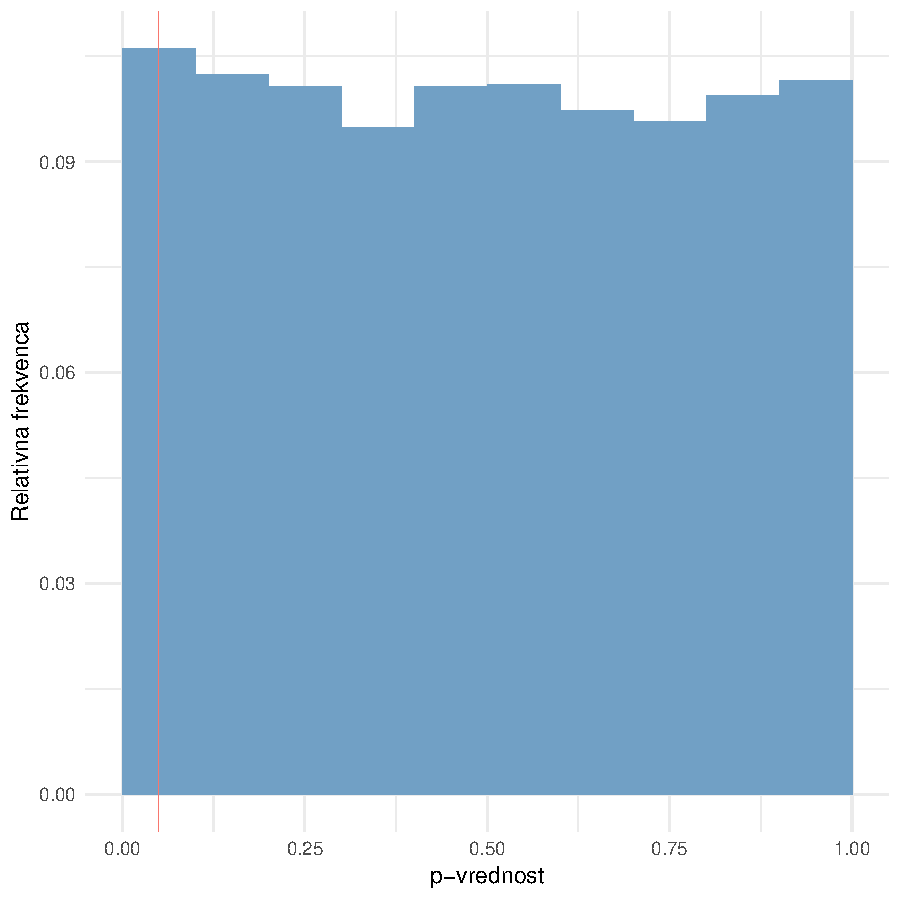
\includegraphics{stadij_H0_M_S1}
    \subcaption{H0}
    \label{fig:1a}
  \end{minipage}%
  \begin{minipage}[b]{.4\linewidth}
    \centering
    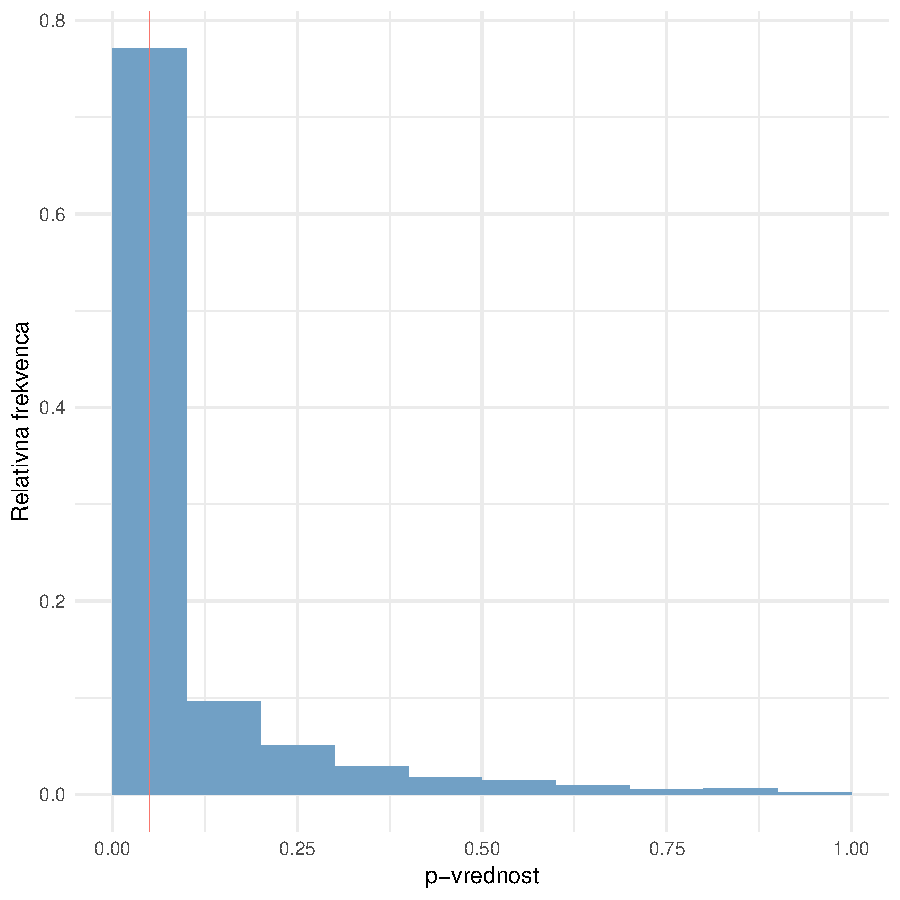
\includegraphics{stadij_HA_M_S1}
    \subcaption{HA}
    \label{fig:1b}
  \end{minipage}
  \caption{Porazdelitve p-vrednosti pridobljenih z LRT glede na hipotezo}
  \label{fig:1}
\end{figure}

% % brejka

\clearpage
\newpage
\subsection{Zaplet}
Pri testiranju z modelom s posameznim zapletom testiramo ali en tip operacije povzroca manj zapletov. Polni model testira enako hipotezo, vendar ob upoštevanju vseh drugih zapletov. V primeru zapletov, ki so neodvisno generirani, vidimo da je težava, ki smo jo izpostavili veliko manj prisotna, oziroma je skladanje z nacinom, ko smo upoštevali posamezne zaplete in ko smo upoštevali vse zaplete, veliko vecje (85\%). Ko testiramo hipoteze pod alternativno hipotezo opazimo, da je moc testa, ko upoštevamo vse zaplete vecja, kot pri modelih s posameznimi zapleti. Seveda pa se zavedamo, da imamo v tem primeru težavo s veckratnim testiranjem hipotez, zato so velikosti p-vrednosti prevelike.

% latex table generated in R 3.5.1 by xtable 1.8-3 package
% Sun May 19 20:22:08 2019
\begin{table}[ht]
\centering
\begin{tabular}{rrrrrrrrrrr}
  \hline
 & Z1 & Z2 & Z3 & Z4 & Z5 & Z6 & Z7 & Z8 & Z9 & Z10 \\ 
  \hline
P(zavrneU) & 0.043 & 0.044 & 0.053 & 0.052 & 0.047 & 0.050 & 0.046 & 0.048 & 0.051 & 0.053 \\ 
  P(zavrneM) & 0.047 & 0.049 & 0.055 & 0.056 & 0.050 & 0.054 & 0.051 & 0.051 & 0.054 & 0.053 \\ 
  P(zavrneU \& zavrenM) & 0.038 & 0.038 & 0.045 & 0.045 & 0.041 & 0.044 & 0.040 & 0.040 & 0.045 & 0.045 \\ 
  P(zavrneM $|$ zavrenU) & 0.866 & 0.878 & 0.851 & 0.851 & 0.872 & 0.878 & 0.858 & 0.838 & 0.884 & 0.856 \\ 
  P(zavrneU $|$ zavrenM) & 0.793 & 0.775 & 0.817 & 0.804 & 0.821 & 0.815 & 0.785 & 0.788 & 0.824 & 0.860 \\ 
   \hline
\end{tabular}
\caption{Verjetnosti zavrnitev pri H0} 
\label{table:6}
\end{table}
% latex table generated in R 3.5.1 by xtable 1.8-3 package
% Sun May 19 20:22:08 2019
\begin{table}[ht]
\centering
\begin{tabular}{rrrrrrrrrrr}
  \hline
 & Z1 & Z2 & Z3 & Z4 & Z5 & Z6 & Z7 & Z8 & Z9 & Z10 \\ 
  \hline
P(zavrneU) & 0.936 & 0.994 & 0.996 & 0.979 & 0.893 & 0.616 & 0.551 & 0.356 & 0.212 & 0.116 \\ 
  P(zavrneM) & 0.930 & 0.987 & 0.999 & 0.997 & 0.965 & 0.786 & 0.722 & 0.506 & 0.289 & 0.112 \\ 
  P(zavrneU \& zavrenM) & 0.929 & 0.986 & 0.996 & 0.978 & 0.885 & 0.589 & 0.519 & 0.314 & 0.158 & 0.065 \\ 
  P(zavrneM $|$ zavrenU) & 0.993 & 0.992 & 0.999 & 0.999 & 0.991 & 0.956 & 0.942 & 0.881 & 0.746 & 0.557 \\ 
  P(zavrneU $|$ zavrenM) & 0.999 & 0.999 & 0.997 & 0.980 & 0.917 & 0.749 & 0.718 & 0.620 & 0.548 & 0.576 \\ 
   \hline
\end{tabular}
\caption{Verjetnosti zavrnitev pri HA} 
\label{table:7}
\end{table}

\newpage
\section{Zakljucek}
Z simulacijami smo primerjali dva nacina testiranja hipotez. Prvic smo testirali tako, da smo za vsako spremenljivko naredili svoj model, drugic pa smo v model vkljucili vse spremenljivke. Teste smo izvedli v dveh primerih, ko so podatki med seboj odvisni in neodvisni. Rezultati naših sklepanj so se skladali s pricakovanimi rezultati. Ugotovili smo torej, da nacin testiranja, ko modeliramo le posamezne spremenljivke ni pravilen in je zavajajoc. Najvecjo napako s takšnim sklepanjem naredimo, ko so spremenljivke med seboj odvisne, v primeru neodvisnih spremenljivk pa je napaka precej manjša (oziroma ujemanje modelov vecje). Kljub vecjem ujemanju nacina testiranje pri neodvisnih podatkih, opazimo, da je moc pri nacini testiranje, ko vkljucimo vse spremenljivke vecja kot pri modelih s posameznimi spremenljivkami. 

\end{document}
